\chapter{Results}
In the next section two error metrics are briefly described, followed by evaluations of each experiment. At the beginning of each section a small description of the problem setting is given, followed by the results and discussion.

\section{Error Metrics}
\label{Emetrics}
For this thesis two error metrics were considered:
\begin{itemize}
  \item \textbf{Point Distance:} Given two meshes with equal topology, meaning both meshes have the same amount of vertices and layout, the error computed is based on the distance between corresponding points. In general, the mean distance is computed over all point correspondences.
  \item \textbf{Face orientations:} The idea behind this method is based on the $\mathbf{Q}$ matrix mentioned in section \ref{faceDeform}. Given two topologically equal meshes, the $\mathbf{Q}$ matrix is computed for all corresponding faces. As it is of interest to investigate the difference in breast shapes, this error tries to quantify the variation of the $\mathbf{Q}$ matrices.
\end{itemize}

One drawback of the point distance method occurs when the two meshes are not aligned properly. This can be solved by applying the same algorithm mentioned in section \ref{align} before computing the error. One advantage of this method is the unit of the error, as it could be converted into a unit of distance, given the distance between two point is known in real world lengths. This error can also be computed when two meshes are not topologically equal by first finding the correspondences between vertices.\\
One advantage of the face orientation method is the invariance of translation and global rotation. This means that moving or rotating the mesh doesn't affect the error. On the other hand, the values of this error don't have a real world meaning and it is a lot harder to apply this method to topologically different meshes, as finding correspondences between faces is a lot more challenging.\\
The methods are depicted in figure \ref{fig:errordiag}. Both methods have their advantages and disadvantages, but due to the fact that alignment isn't a problem, the error metric used in this thesis is the point distance method.

\begin{figure}
\centering
\begin{subfigure}{.5\textwidth}
  \centering
  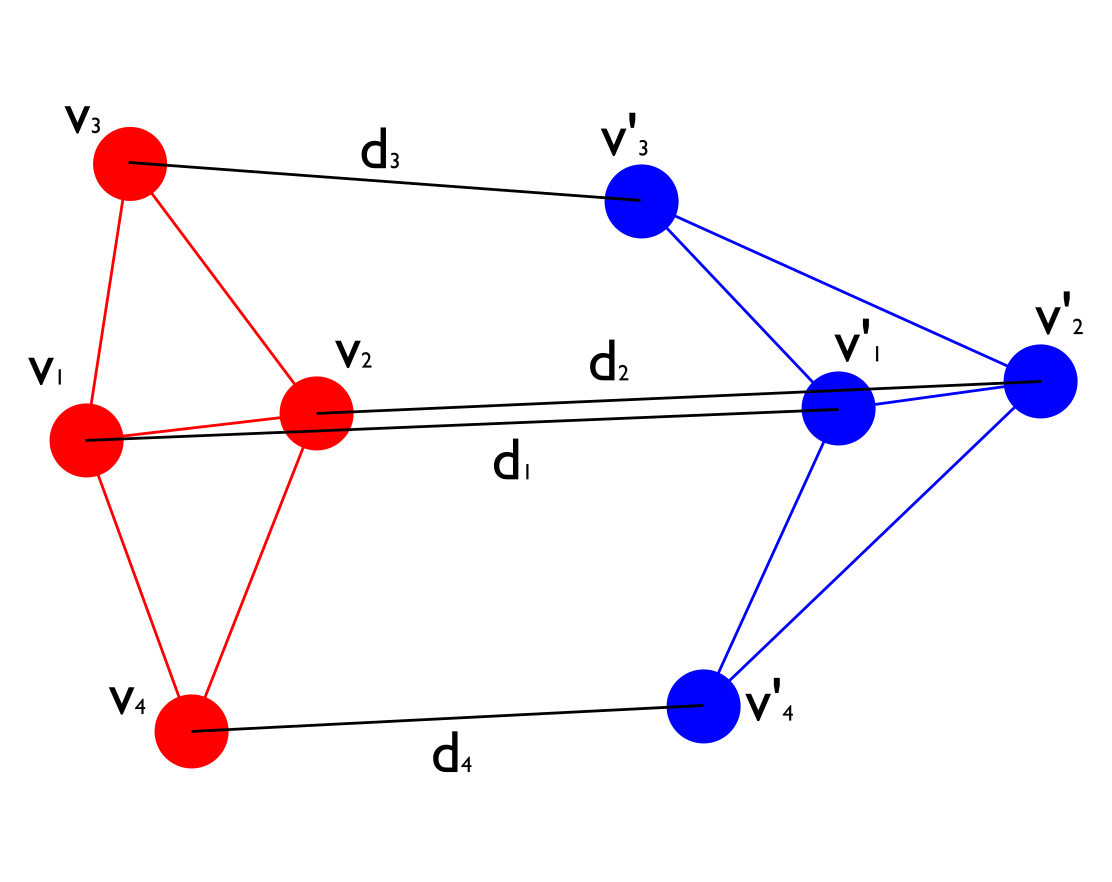
\includegraphics[width=.75\linewidth]{figures/pediag}
\end{subfigure}%
\begin{subfigure}{.5\textwidth}
  \centering
  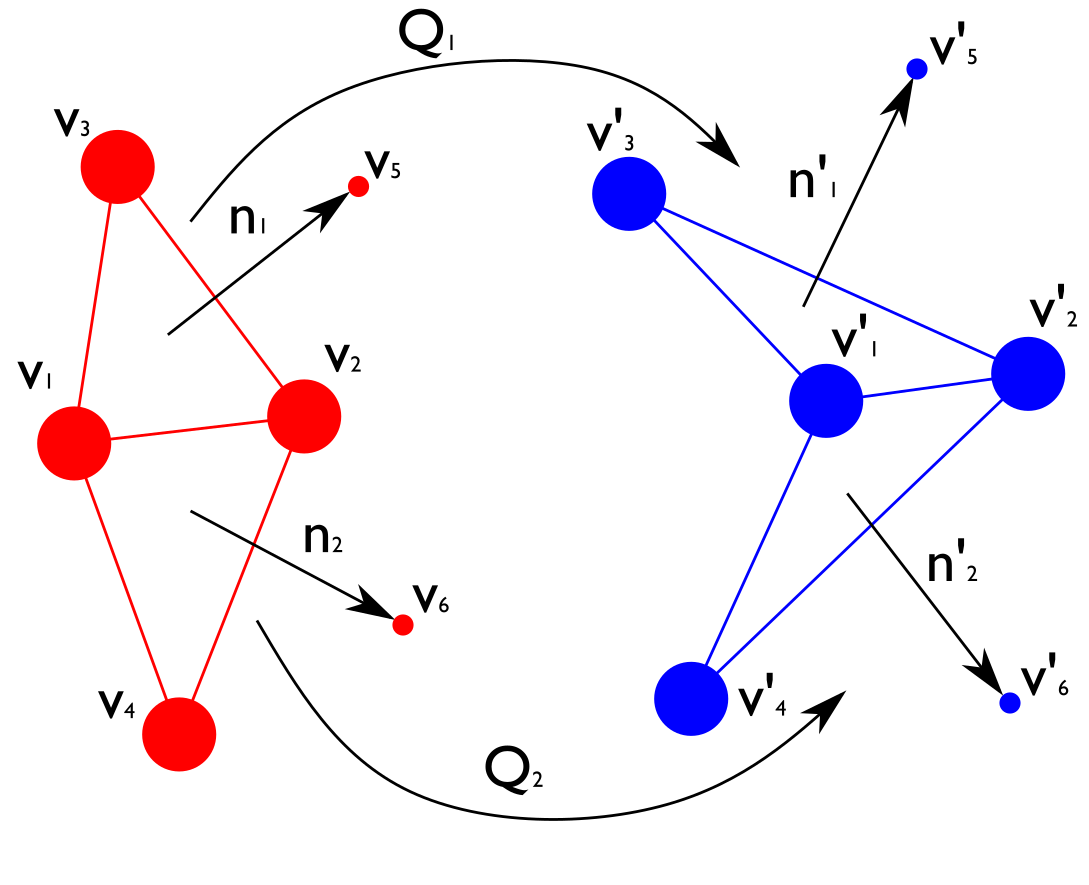
\includegraphics[width=.75\linewidth]{figures/dediag}
\end{subfigure}
\caption{The left image depicts distances between corresponding points of the mesh. The right image shows a representation of the information used to compute the $\mathbf{Q}$ matrix.}
\label{fig:errordiag}
\end{figure}

\section{Evaluation}
In the following section the evaluation methods, that were used, are explained. Optimally, when evaluating a prediction some representation of the true outcome, often called the "ground truth", is given. This is useful to quantify how acurate the prediction was.
\subsection{Mesh Point Error} % Compare to GT
\label{mpError}
For this method the comparison is done as explained in section \ref{Emetrics}. Before evaluating the point distances between a prediction and the ground truth, the meshes are aligned as mentioned in section \ref{align}. Additionally, the mean point distance error is computed by diving by the number of vertices in the mesh and also by diving by the diagonal of the largest bounding box over all examples to scale the error to a meaningful unit. Given a prediction of a mesh $M^{(p)}$ and the ground truth $M^{(g)}$ the problem can be stated as:
\begin{gather}
error = \frac{1}{nd_{max}}\sum_{i=1}^{n} \sqrt{\sum_{j=1}^3(M_{i,j}^{(p)} - M_{i,j}^{(g)})^2}
\end{gather}
where $n$ is the number of vertices of the mesh, $d_{max}$ is the diagonal length of the largest bounding box over all examples and the final result is a scalar value.
\subsection{Error Heat Map} % Compare to NRICP vs Ceres
\label{mhError}
The idea of this method is to generate a visualization of the error, indicating where the prediction failed to represent the ground truth the most. This can be accomplished by computing the error described in section \ref{Emetrics} but instead of adding up the errors keeping them separate for each vertex. This error per vertex is accumulated over multiple samples. Given the  k-th prediction of a mesh $M^{(p_k)}$ and the corresponding ground truth $M^{(g_k)}$ the problem can be described as:
\begin{gather}
e'_{i} = \sum_{k=1}^{m} \sqrt{\sum_{j=1}^3(M_{i,j}^{(p_k)} - M_{i,j}^{(g_k)})^2} \  \forall i=1 \dots n \text{ with } e = \frac{e'}{max(e')}
\end{gather}
where $m$ is the number of samples, $e'$ is a vector of the accumulated errors over all samples and $e$ is a vector of the errors scaled by the largest entry in $e'$. This is done to visualize the error on a range, such that, for example the error can be color coded where red is equivalent to a large error and green is a small error.
%TODO change colors used for large and small according to colormap used
\section{Input Data for PCA}
In this experiment three different variations of data inputs are tested for PCA as described in section \ref{paramModel} and the following two subsections. Based on the resulting parameters of each model, a linear mapping is created and compared based on the error of the predictions.

\subsection{Problem Setting}
Given a data set comprised of 57 pairs of meshes where one mesh is based on the before point cloud and the other is based on the after point cloud. Both sets are split into equally sized sets of 42 training pairs and 15 testing pairs. Each variation is trained on the training set and afterwards evaluated on the test set. The evaluation is done by computing a linear mapping over the parameters of each model. Then the mean mesh point error over all 15 testing pairs is computed and a error heat map is generated.
\subsection{Results}
In the table \ref{tablePDN} the time column is the amount of time each method needed to compute the parameteric model. The training mean error is computed as mentioned in \ref{mpError} for each case. The mean is computed over all cases. The same is done for the test mean error. In each subfigure in figure \ref{fig:PDNheatmap} the values that are listed above are the respective $\mathbf{max(e')}$ as explained in \ref{mhError}. Additionally, one vertex on the border doesn't have a colored point as the error wasn't being computed corretly for it.

\begin{table}[]
\centering
\label{tablePDN}
\begin{tabular}{l|l|l|l|l|}
\cline{2-5}
                                                  & \textbf{Time} & \textbf{\begin{tabular}[c]{@{}l@{}}Training\\ Mean Error\end{tabular}} & \multicolumn{2}{l|}{\textbf{\begin{tabular}[c]{@{}l@{}}Test\\ Mean Error\end{tabular}}} \\ \hline
\multicolumn{1}{|l|}{\textbf{Point}}              & 0.06s         & 0.00733                                                                & \multicolumn{2}{l|}{0.01845}                                                            \\ \hline
\multicolumn{1}{|l|}{\textbf{Deformation}}        & 6.81s         & 0.0090                                                                 & \multicolumn{2}{l|}{0.02795}                                                            \\ \hline
\multicolumn{1}{|l|}{\textbf{Points and Normals}} & 2.92s         & 0.0071                                                                 & \multicolumn{2}{l|}{0.01841}                                                            \\ \hline
\end{tabular}
\caption[Table of results of Input Data for PCA]{Results in terms of mean mesh point error are listed for the training and for the test set. Also the time each function took to compute the parametric model is listed in seconds.}
\end{table}

\begin{figure}
\centering
\makebox[\textwidth][c]{%
  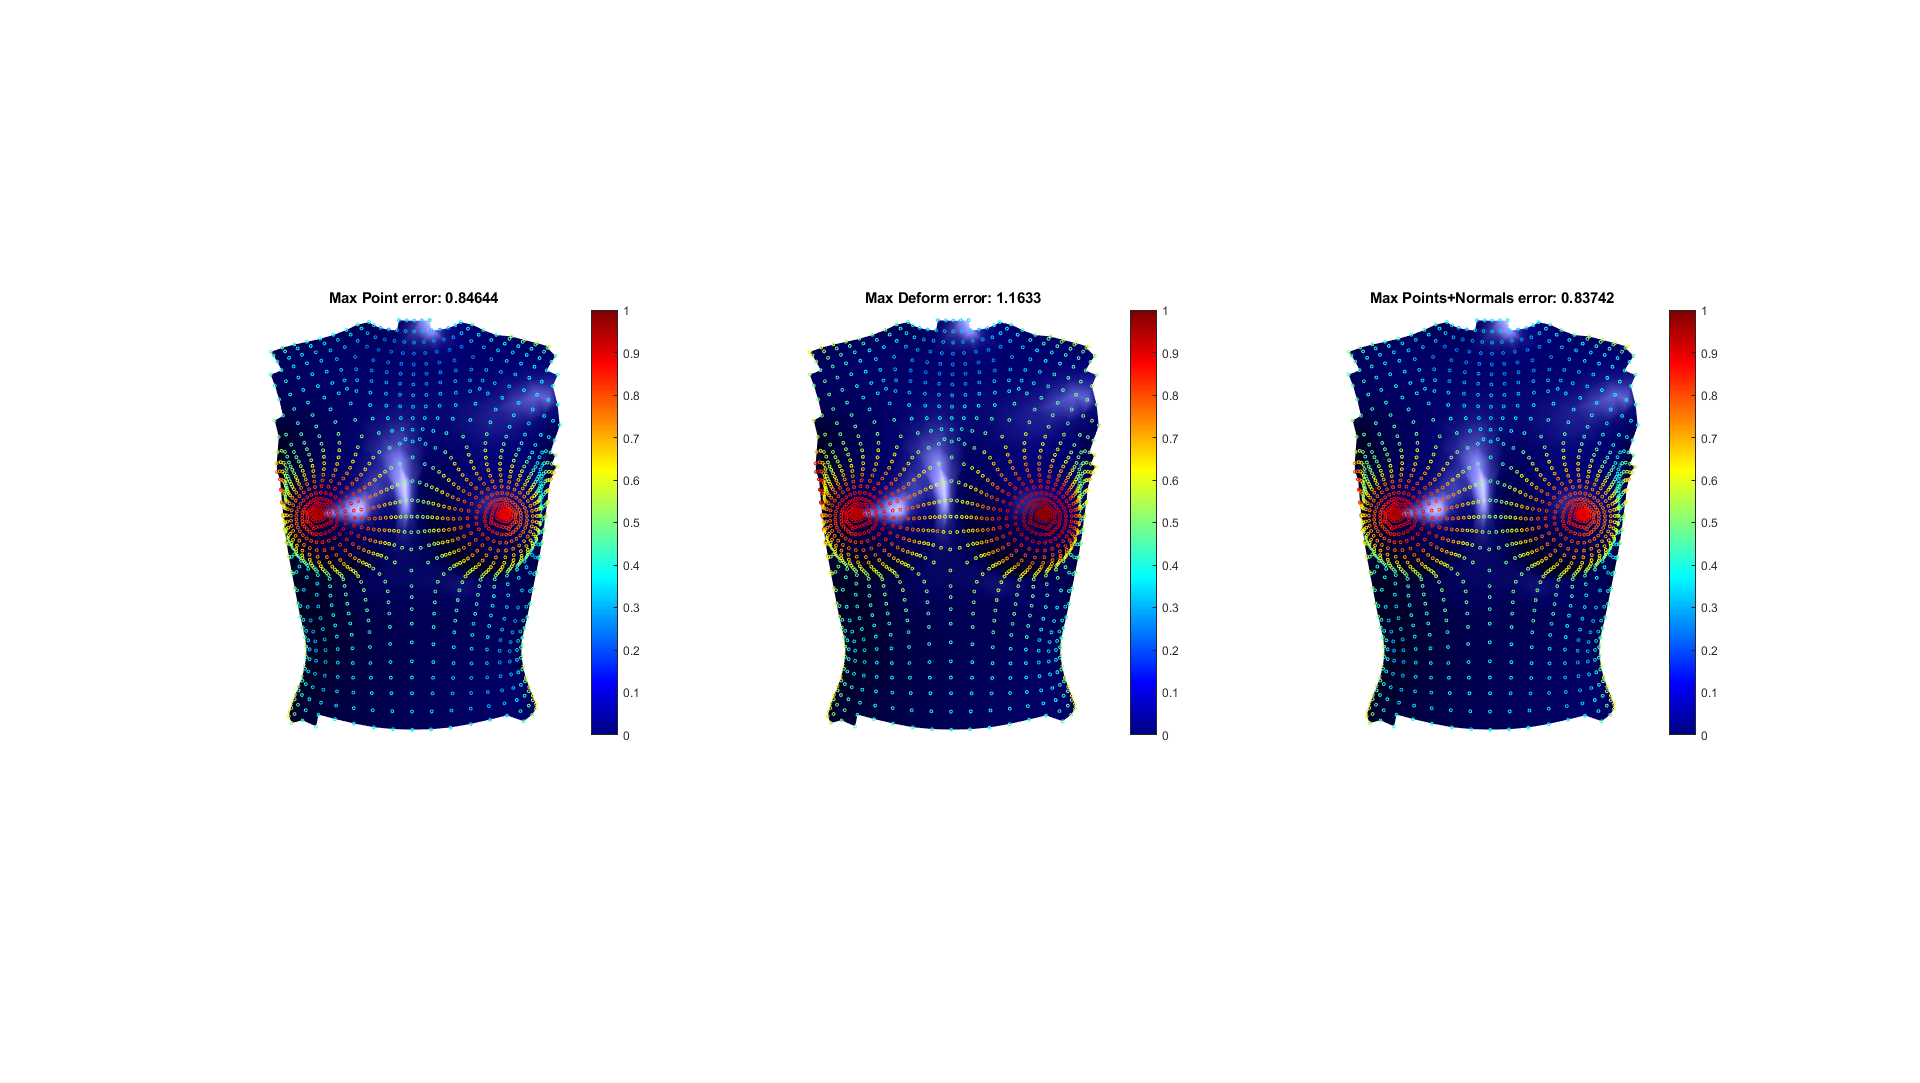
\includegraphics[width=1.6\textwidth]{figures/evalPDN}%
}
\caption[Input Data for PCA error heat map]{The left image shows the error heat map when using the point method. The middle one uses the deformation method. The right one uses point and normals. The color of each point reflects the amount of the error. Red color indicates large error, blue small error.}
\label{fig:PDNheatmap}
\end{figure}

\subsection{Discussion}
The amount of time it takes to compute the parameteric model based on deformations takes a lot longer due to the fact that additional normals need to be computed followed by the computation of the $Q$ matrix. One can see that the additional time to compute normals is also reflected in the point and normals method. Therefore roughly $\mathbf{40\%}$ of the time is accounted for by the normal computation.\\
All three methods worsen going from training to test case, but that is expected. This is caused by the models having seen the training set before and are already familiar with those examples. Of the three methods the points and normals method achieves the best results over test and training. The reason this occurs is due to the fact that the the normals carry some information of the size of the faces.

\section{Learning Mapping}
The next step was to investigate, if non-linear mappings could perform better than a linear mapping. Additionally, it is checked how the error changes, when PCA is done on the complete set, instead of, only the training set. The reason, this is done, is because the mapping shouldn't be penalized or perform badly because of the parametric model. For each of the approaches the best parameters need to be found first by running cross-validation grid search. Each of the learnt mappings can be applied to the test set and compared against the ground truth. The mean point error is computed to measure the error.

\subsection{Problem Setting}
The parameters for each of the 57 pair meshes are computed according to two parametric model. These will be referred to as the "complete" and "incomplete" model, where the "complete" model was based on the training and test data, where as the "incomplete" model only received the training data. The non-linear approaches used are a decision tree regressor, a random forest regressor, a multilayer perceptron with a rectified linear unit (ReLU) as its activation function and a multilayer perceptron without a ReLU. \\
For each approach the best parameters are evaluated by running cross-validation grid search for either cases. Finally, the training and test errors are computed based on the best parameters and a ratio between test and training error is calculated. Optimally, this ratio should be one, as the test error should be equally low as the training error.

\subsection{Results}
The results for the different cases can be seen in \ref{tableMapping}. The table is divided into two sections, the first half for the results of the "incomplete" model and the second for the "complete" model. The first row of results are the mean errors for the training set, the second row for the test set. The error for a prediction is computed by comparing to the ground truth with the mesh point error as explained in \ref{mpError}. The resulting error is equivalent to the mean over all errors. The last column is the ratio between test and training.
\begin{table}[]
\centering
\label{tableMapping}
\begin{tabular}{l|l|l|l|l|}
\cline{2-5}
\textbf{PCA Model}  & \textbf{Method}        & \textbf{\begin{tabular}[c]{@{}l@{}}Training\\ Mean Error\end{tabular}} & \textbf{\begin{tabular}[c]{@{}l@{}}Test\\ Mean Error\end{tabular}} & \textbf{Ratio\\ Test/Train} \\ \cline{2-5}
\textbf{Incomplete} & \textbf{Linear}        & 0.0073                                                                 & 0.0184                                                             & 2.52                     \\ \cline{2-5}
\textbf{}           & \textbf{Random Forest} & 0.0068                                                                 & 0.0196                                                             & 2.88                     \\ \cline{2-5}
\textbf{}           & \textbf{Decision Tree} & 0.0127                                                                 & 0.0237                                                             & 1.86                     \\ \cline{2-5}
\textbf{}           & \textbf{MLP}           & 0.0154                                                                 & 0.0186                                                             & 1.21                     \\ \cline{2-5}
\textbf{}           & \textbf{MLP ReLU}      & 0.0173                                                                 & 0.0203                                                             & 1.17                     \\ \cline{2-5}
\textbf{Complete}   & \textbf{Linear}        & 0.0076                                                                 & 0.0357                                                             & 4.70                     \\ \cline{2-5}
\textbf{}           & \textbf{Random Forest} & 0.0077                                                                 & 0.0196                                                             & 2.55                     \\ \cline{2-5}
\textbf{}           & \textbf{Decision Tree} & 0.0125                                                                 & 0.0218                                                             & 1.74                     \\ \cline{2-5}
\textbf{}           & \textbf{MLP}           & 0.0152                                                                 & 0.0193                                                             & 1.27                     \\ \cline{2-5}
\textbf{}           & \textbf{MLP ReLU}      & 0.0161                                                                 & 0.0193                                                             & 1.20                     \\ \cline{2-5}
\end{tabular}
\caption[Learnt mapping results]{This tables shows the mean errors computed on the training and test set. The first five rows show the results for the "incomplete" model, the last five for the "complete" model. The first two columns are the training and test error, followed by the ratio of test to training error.}
\end{table}

\subsection{Discussion}
It is interesting to see that the training error of the linear method and the random forest increases slightly going from the "incomplete" to the "complete" model. This must be caused by some examples in the test set being similar to some of the examples in the training set and forcing the parameters to adjust. The other three methods improve slightly in terms of training error due to the "complete" model. Independant of case, the test error is always larger than the training error. This is expected and was already discussed above.\\

The behaviour of the test error going from "incomplete" to "complete" is similar to the training error. The linear method worsens gravely, perhaps due to the "complete" model describing a wider space, making it harder for the linear method to find an appropriate mapping. All of the non-linear methods perform similarly in the "complete" case compared to the "incomplete" case in terms of mean test error.\\

Even though the best performing method in terms of error is the MLP, the MLP with ReLU has similar error values but has a slightly better test/train ratio. This could indicate that this method is more robust, meaning that the error behaves similarly when applied to new data.

\section{Parametric Models}
Given two parametric models and a test set of point clouds, both models process the point clouds as described in section \ref{fitModel}.
\subsection{Problem Setting}
\subsection{Results}
\subsection{Discussion}

\chapter{Conclusion}

\section{Outlook}
